\documentclass[10pt, journal]{IEEEtran}
\usepackage{amsmath}
\usepackage{amsfonts}
\usepackage{amssymb}
\usepackage{hyperref}
\usepackage{graphicx}
\graphicspath{ {images/} }
\usepackage[caption=false,font=footnotesize]{subfig}

\DeclareMathOperator{\vol}{Vol}

\title{Object Detection in Scientific Images (DRAFT)}

\author{Benjamin Killeen and Gordon Kindlmann %
  \thanks{Benjamin Killeen is an undergraduate with the Department of Computer
    Science, University of Chicago, Chicago, IL 60637, USA (email:
    \href{mailto:killeen@uchicago.edu}{killeen@uchicago.edu})} %
  \thanks{Gordon Kindlmann is with the Department of Computer Science, 
    University of Chicago, Chicago, IL 60637, USA (email:
    \href{mailto:glk@uchicago.edu}{glk@uchicago.edu})} %
}
\begin{document}
\maketitle

\begin{abstract}
  Together with large training sets, Deep Neural Networks (DNNs) have enabled a
  wide range of advancements in Computer Vision tasks, especially with regard to
  object detection in real-world images. Object detection for scientific images,
  on the other hand, presents challenges unlike typical vision tasks. Scientific
  tasks exhibit \emph{governing principles} (GPs) in their datasets, which
  result from the phenomena under investigation. In this progress report, we
  describe our ongoing effort toward training DNNs which are agnostic to
  governing principles yet perform reliably on scarce data.\footnote{Code
    available at \href{https://github.com/bendkill/artifice}
    {github.com/bendkill/artifice}}
\end{abstract}

\section{Introduction}
\label{sec:introduction}

% TODO: incorporate principle of governing principles.

Imaging systems are a vital component of many scientific experiments, used as
the primary measuring device of properties like object location or
orientation. In cases where no alternative measuring device exists, accurate
labeling is of the utmost importance. However, such image analysis can prove
labor-intensive. Traditional methods involve \emph{ad hoc} solutions suited for
one experimental setup even though more general object detection tasks have been
well-studied in Computer Vision. In this report, we introduce an ongoing effort
to generalize principles for image-data analysis across scientific tasks using
DNNs, emphasizing the importance of careful data augmentation.

Deep Neural Networks\footnote{Alternatively, deep convolutional neural networks}
have shown remarkable success on real-world tasks
\cite{krizhevsky_imagenet_2012}, such as challenges for datasets like ImageNet
\cite{deng_imagenet:_nodate} and COCO \cite{lin_microsoft_2014}. These and other
data underlie supervised learning approaches, as in
Fig. \ref{fig:traditional-graph}, for increasingly complex tasks. Scientific
experiments, on the other hand, have no dataset except what they generate; each
experiment constitutes its own unique task, sometimes entirely disjoint from
established datasets. The man-hour investment required for labeling scientific
images motivates approaches such as active learning \cite{settles_active_2012,
  kao_localization-aware_2018, jain_active_2016} and data augmentation,
\cite{krizhevsky_imagenet_2012, ronneberger_u-net:_2015}. The focus of this
report, however, is the application of boundary-aware augmentation, which aims
to reduce overfitting to governing principles (section
\ref{sec:governing-principles}).

\begin{figure*}
  \centering
  \subfloat[]{
    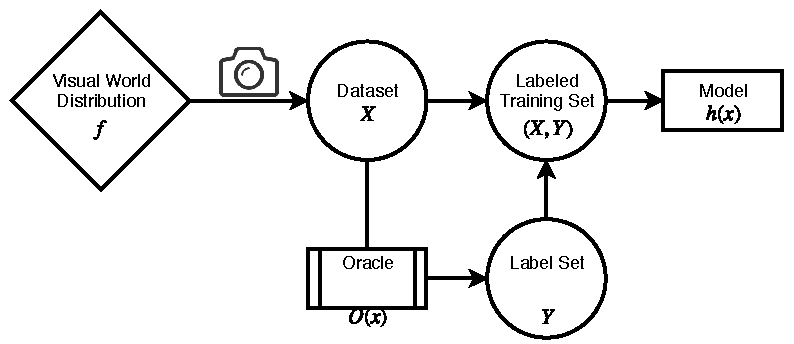
\includegraphics[width=0.46\linewidth]{traditional_graph}
    \label{fig:traditional-graph}
  }
  \hfill
  \subfloat[]{
    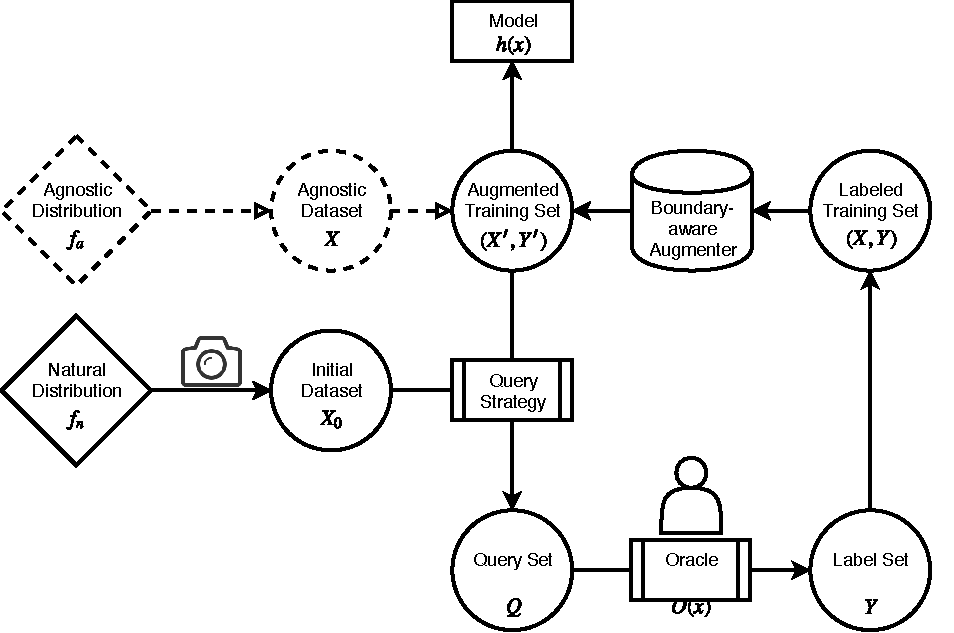
\includegraphics[width=0.50\linewidth]{artifice_graph}
    \label{fig:artifice-graph}
  }
  \caption{During supervised learning for real-world vision tasks \textbf{(a)},
    a camera samples a large dataset $X$ from the ``visual world'' distribution
    $f$. For scientific tasks \textbf{(b)}, an experiment samples a small
    initial dataset $X_0$ from the natural distribution $f_n$, which includes
    the effects of any governing principles. Our proposed training method
    incorporates a boundary-aware augmenter $A$, which uses the training set
    $(X,Y)$ to simulate drawing examples from the agnostic distribution
    $f_a$. Dashed lines indicate theoretical or simulated objects.}
  \label{fig:dependency-graphs}
\end{figure*}

\subsection{Governing Principles}
\label{sec:governing-principles}

Scientific experiments use images as a measuring technique, recovering
properties like object position or orientation for further analysis. These
quantities encode the underlying structure of the experiment, if any exists,
which is under investigation. Images of a sphere in free-fall, for example,
capture the laws of gravity, which any measurement \emph{aiming to study
  gravity} ought to ignore for the sake of scientific rigor. Experiments that
anticipate such \emph{governing principles} (GPs) in the data commit a logical
fallacy by assuming the initial point. This observation is particularly
important for training DNNs in scientific tasks. Like any statistical model,
DNNS are prone to overfitting when underlying correlations are present. In order
to address this issue, we contrast scientific tasks with traditional tasks in
computer vision.

Fig. \ref{fig:traditional-graph} outlines the training process for traditional
vision tasks. Typically, such approaches leverage a large, fully labeled
training set $(X,Y)$, \textit{e.g.} ImageNet, where $X$ is the set of
$M\times N$ images and $Y\subseteq \mathbb{R}^n$ is the label set. In any task,
the labeling comprises a lower-dimensional representation of the data space,
encoding valuable information from each example. $n$ denotes the dimensionality
of the labeling, \textit{e.g.} the number of classes. Supervised learning aims
to train a model (such as a DNN)
$h : \mathbb{R}^{M\times N} \rightarrow \mathbb{R}^n$ that can interpret the
visual world. Crucial, the visual world is not a uniformly distributed set of
images; we denote its probability distribution as
$f : \mathbb{R}^{M\times N} \rightarrow \mathbb{R}$, from which every dataset
draws examples as independently and identically distributed as possible.

For real-world tasks, sampling $f$ in this manner is desirable, but in
scientific tasks, governing principles make sampling from the original
distribution undesirable. In fact, for the purposes of training, we wish to
sample from a distribution as uniform as possible in the label space
$\mathbb{R}^n$. That is, we wish for the dataset $X$ to correspond to labels $Y$
which contain almost no structure, within reasonable boundaries. Fortunately,
most scientific experiments have well-known boundaries incorporated into their
design. A sphere in free-fall, for instance, might be bound to one-dimension by
a track, even though its image-space position is described by two
coordinates. Fig. \ref{fig:gyros} shows an experiment where dot markers are
confined to a small circular region. These \emph{label-space boundaries} are a
low-dimensional representation of a data-space region
$\chi \subseteq \mathbb{R}^{M\times N}$ such that the real distribution $f$
obeys
\[ (\forall x \not\in \chi)(f_n(x) = 0). \] Even with perfect knowledge of these
boundaries, however, it is difficult or impossible to recover $\chi$ from the
lower-dimensional label-space boundaries.

Although $\chi$ is largely a theoretical construct, it serves as a useful
concept for training GP-agnostic models. Consider the uniform distribution
across it, which we will refer to as the \emph{agnostic distribution}:
\[ f_a(x) =
  \begin{cases}
    \frac{1}{\vol(\chi)} & x \in \chi \\
    0 & x \not\in \chi
  \end{cases}
\] From the initial dataset $X_0$, then, we wish to generate and label an
augmented dataset $X$ that approximates a GP-agnostic dataset $X_a \sim f_a$. In
this report, we introduce a \emph{Boundary-Aware Augmenter} (BAA) that utilizes
label-space boundaries and instance segmentations to approach $X_a$.

\section{Related Work}
\label{sec:related-work}

% \cite{bernardis_finding_2010} uses a graph-cut approach for dot localization,
% noting various scientific applications, and \cite{ronneberger_u-net:_2015}
% applies a DNN for semantic segmentation of neuronal structures in electron
% microscope stacks.

The problems of data scarcity and biases are well-considered in computer
vision. \cite{torralba_unbiased_2011} explores bias in popular datasets for
computer vision by training DNNs on one dataset but testing them on another
(employing a test-train split for fairness). Unsurprisingly, networks perform
best on the dataset for which they were trained, even though datasets like
ImageNet aim to capture the unbiased visual world. Creating unbiased datasets
for real-world vision tasks remains an open problem, one which may demand a
reckoning for the community's focus on dataset performance scores.

\cite{ronneberger_u-net:_2015} describes a novel segmentation architecture using
up-convolutions which, paired with their data augmentation scheme, performs well
on biomedical images taken from electron stacks. Like our approach,
\cite{ronneberger_u-net:_2015} confronts data scarcity but also focuses on
applications in biomedical imaging, where semantic segmentation is often
sufficient. We aim to address scientific tasks more generally, using semantic
segmentation as one component of a general detection system, capable of
recovering location, orientation, or shape for multiple objects. Capturing these
quantities with minimal human effort would accelerate a wide range of scientific
experiments.

\begin{figure}
  \centering
  \subfloat[Gyroscopic Model]{
    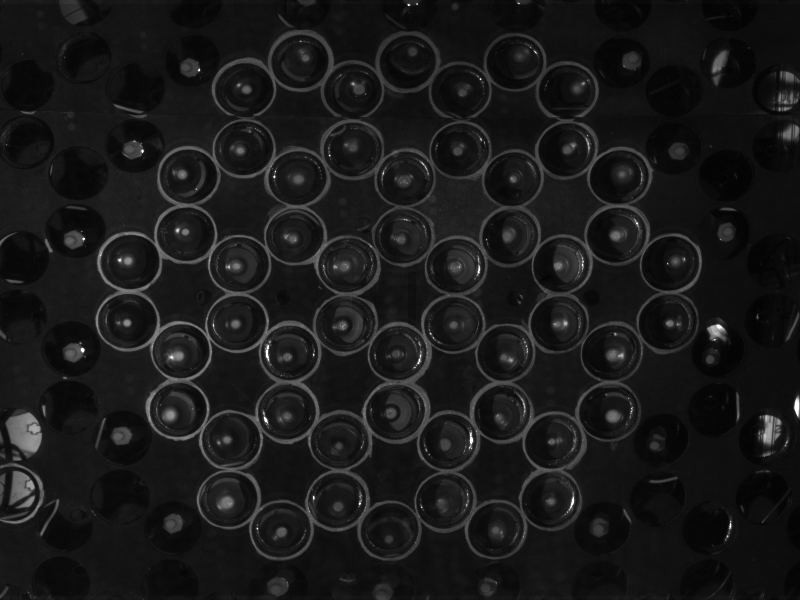
\includegraphics[height=0.37\linewidth]{gyros}
    \label{fig:gyros}
  }
  \hfill
  \subfloat[Coupled Spheres]{
    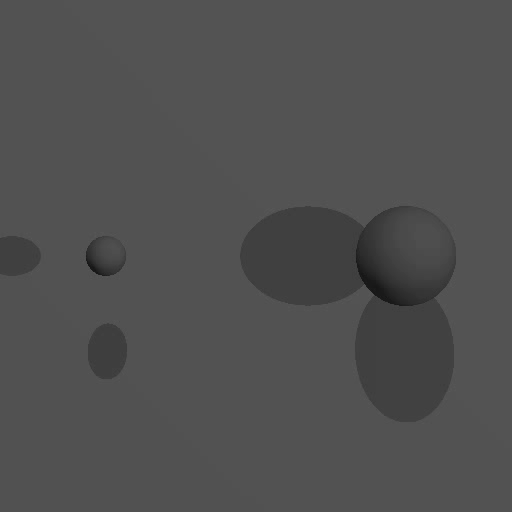
\includegraphics[height=0.37\linewidth]{coupled_spheres}
    \label{fig:coupled-spheres}
  }

  \caption[example experiments]{Example images from scientific experiments:
    \textbf{(a)} gyroscopic model for topological metamaterials
    \cite{nash_topological_2015}. Each dot is bound inside the circle
    surrounding it. \textbf{(b)} still frame from a simulated experiment of two
    spheres coupled by an invisible spring. Full video \href
    {https://github.com/bendkill/artifice/blob/master/docs/coupled_spheres.gif}
    {here}.}
  \label{fig:example-experiments}
\end{figure}

\section{Method}
\label{sec:method}

TODO: UPDATE METHOD

Fig. \ref{fig:artifice-graph} shows our training scheme at a high-level. The
details of this scheme are an area of active inquiry, with open questions
pertaining to the \emph{selector}, for active learning; the \emph{augmenter},
which should incorporate the experiment's imposed constraints; and the model
$f$, which employs one or more DNNs.

Because of the variety of scientific tasks, $f$ must remain flexible with regard
to its output. Toward this end, we envision a two-step procedure which (1)
obtains an instance segmentation \cite{ronneberger_u-net:_2015, bai_deep_2016}
for objects of interest and (2) learns the target parameters (location,
orientation, etc.) for each object. Whether these steps occur in an end-to-end
fashion or are divided between several training steps is an open question. We
do, however, consider (1) to be a vital step for the sake of maintaining
generality. Even in scientific tasks where segmentation is unneeded, such as the
Coupled Sphere experiment in \ref{sec:method}, obtaining pixel-level masks of
each object enables more advanced data augmentation methods.

Because we wish to minimize the man-hours required for training as much as
possible, we use an active learning scheme to select a query set
$Q \subseteq X'$ which will most inform training. The application of active
learning to semantic segmentation has received relatively little attention, with
the exception of \cite{vezhnevets_active_2012}, and the added complication of an
imperfect labeler remains an open question in the field
\cite{settles_active_2012}. We aim to address both issues with its
\emph{selector}.

Finally, the \emph{augmenter} will incorporate both the semantic segmentations
obtained by $f$ and the imposed constraints specified by the experimenter to
improve training as much as possible. We hope to test many augmentation methods
while keeping in mind that the image space of a scientific task is usually much
more constrained than that of a real-world
task. \cite{krizhevsky_imagenet_2012}, for instance, uses sub-image extraction,
flipping, and PCA analysis of RGB channels to augment ImageNet. These methods
are not necessarily applicable to scientific tasks, where imposed constraints
might invalidate a flipped image, for instance.

\section{Simulated Experiments}
\label{sec:simulated-experiments}

TODO: UPDATE SIMULATED EXPERIMENTS

In order to show our method's effectiveness, we develop several virtual
experiments. These simulations offer several advantages over images from real
experiments, such as in Fig. \ref{fig:gyros}. First, we have perfect knowledge
of the experiment's ``Truth'' $\tilde{Y}$, as opposed to imperfect measurements,
or ``ground truth,'' $Y$. In well established datasets, $\tilde{Y}$ and $Y$ are
nearly identical, but we must rely on one or a few human labelers for what
should be unambiguous quantities. For testing, we calculate $\tilde{Y}$ from the
known parameters of the simulation, and we emulate a human labeler by
introducing small perturbations to $\tilde{Y}$, producing $Y$. Part of
our goal is to train a DNN with predictions $\hat{Y}$ that more closely
approximate $\tilde{Y}$ than the labels $Y$. Simulated experiments allow us to
test this performance.

Fig. \ref{fig:coupled-spheres} shows one such experiment. In this case, two
spheres with different masses rotate in free space, coupled by an invisible
spring. The goal of the Coupled Spheres experiment is to recover physical
properties of the spring using $(x,y)$ positions of the two spheres. Imposed
constraints include the $z$-coordinate of each sphere, which is set to the
image-plane, as well as each sphere's apparent size. Inherent constraints
include the physical properties of the spring, \textit{e.g.} the spring constant
and relaxed length. Adverse noise, which in this case includes any shadows,
lighting effects, and possible occlusion, also presents a challenge for
detection.

To demonstrate our method's resilience to inherent constraints, we intend to
train a DNN on one experiment and evaluate its performance on experiments with
different simulated springs. This simple example illustrates the general
resilience that we wish to develop.

\section{Conclusion}
\label{sec:conclusion}

TODO: CONCLUSION

\section*{Acknowledgment}
\label{sec:acknowledgment}

Thanks to Michael Maire for input and guidance, as well as William Irvine for
access to image data from his laboratory.

\bibliographystyle{IEEEtran}
\bibliography{IEEEabrv, artifice}

\end{document}
%%% Local Variables:
%%% mode: latex
%%% TeX-master: t
%%% End:
